%!TEX root = ../main.tex
\doublespacing
\chapter{Measuring Source Sizes in Visibility Space}
\label{chap:measuring_source_sizes}

Low frequency radio wave scattering and refraction can have a dramatic effect on the observed size and position of radio sources in the solar corona.
The scattering and refraction is thought to be due to fluctuations of electron density caused by turbulence. Hence, determining the true radio source size can provide information on the turbulence in coronal plasma.
However, the lack of high spatial resolution radio interferometric observations at low frequencies such as with the LOw Frequency ARray (LOFAR) have made it difficult to determine the true radio source size and level of radio wave scattering.
Here we directly fit the visibilities of a LOFAR observation of a type IIIb radio burst with an elliptical Gaussian to determine its source size and position. This circumvents the need for imaging of the source followed by deconvolution, which can introduce spurious effects on source size and shape.
For a burst at 34.76~MHz, we find a full width at half maximum height (FWHM) along the major and minor axes to be 18.8~arcmin~$\pm~0.1$~arcmin and 10.2~arcmin~$\pm~0.1$~arcmin respectively at a plane of sky heliocentric distance of 1.75~R$_\odot$.
Our results suggest that the level of density fluctuations in the solar corona  is  the  major  cause  of  the  scattering  of  radio  waves, resulting in  large  source  sizes. However, the magnitude of $\varepsilon$ may be smaller than previously derived in comparison to observations of radio wave scattering in tied-array images. This work was published as \cite{Murphy2021} in \textit{Astronomy and Astrophysics}.

\section{Introduction} \label{sec:intro}
Low frequency radio wave propagation in the solar corona is not fully understood. It is widely accepted that scattering of radio waves off of density inhomogeneities plays a key role in the observed source sizes of radio bursts \citep{Fokker1965,Steinberg1971,Stewart1972,Riddle1974,Thejappa2007,Thejappa2008,Kontar2019}. However, the exact extent to which observed source sizes are broadened is difficult to measure as it requires an angular resolution to spatially resolve the source as well as an \textit{a priori} knowledge of its original size.
Current generation radio interferometers such as the LOw Frequency ARray \citep[LOFAR;][]{VanHaarlem2013} have the resolving power to observe this angular size. This angular resolution can be exploited to accurately determine burst size and position, both of which are indicators of the level of radio scattering in the corona, which in turn is related to the level of turbulent density fluctuations. Hence a better understanding of scattering may lead to new insights into the nature of coronal turbulence.

The study of radio wave scattering in the solar corona has its origins in the 60s and 70s. \cite{Fokker1965}, \cite{Steinberg1971}, \cite{Stewart1972} and \cite{Riddle1974} did seminal work on ray tracing of radio waves in various coronal models. All concluded that sources emitted near the plasma frequency in the solar corona are enlarged due to scattering of radio waves from coronal density fluctuations. While the explanation of coronal scattering for observed source characteristics fell out of favour by the mid 1980s \citep{McLean1985}, it has seen renewed interested in low frequency radio observations in recent years  \citep{Thejappa2007,Thejappa2008,Kontar2017,Sharykin2018,Gordovskyy2019,Kontar2019}.

In low frequency imaging, the extent of scattering in the corona can be determined through the analysis of type III radio bursts, particularly their position and size in images or decay times in dynamic spectra \citep[e.g.][]{Kontar2019, Gordovskyy2019, Krupar2018}. Given that these bursts are due to plasma emission from electron beams propagating through coronal plasma \citep[see][for a review]{Reid2014}, they provide a density diagnostic of such plasma. In particular, a subset of these bursts known as ``type IIIb" (see Section \ref{sec:typeIII}) provide a diagnostic of scattering in coronal plasma due to density fluctuations from turbulence. For example, type IIIb bursts often show fine structures or ``striae" along the burst envelope \citep{Ellis1967,Ellis1969,DeLaNoe1972,DeLaNoe1975,Melnik2010b}, which are believed to be caused by density inhomogeneities in the corona \citep{Takakura1975}. Using a density model, the frequency bandwidth of these striae can be used to infer the vertical extent of the density inhomogeneity in space. A comparison of this spatial extent to observed source size in images can provide the extent to which the radio emission has been scattered \citep[e.g.][]{Kontar2017}.

Theoretically, the extent of scattering in the corona is related to the root mean squared (rms) fluctuations of electron density $\varepsilon = \sqrt{\left< \delta n^2 \right>}/n$. Many recent works have assumed a value for $\varepsilon$ to use in simulations in order to recreate the time profile and source size of solar radio bursts \citep[e.g.][]{Krupar2018, Kontar2019}. However, few use the observed source size and time profile to determine $\varepsilon$. Those that have are limited to determining the value of $\varepsilon$ in the solar wind at distances $> 10 \, R_\odot$. Techniques such as interplanetary scintillations \citep[e.g.][]{Bisoi2014} and Crab nebula occultation \citep{SasikumarRaja2016} have also been used to determine $\varepsilon$ at these distances. The general conclusion of these studies is that $\varepsilon$ varies slowly with heliocentric distance and has typical values of $0.001 \lesssim \varepsilon \lesssim 0.02$ in the range of 10 to 45 $\, R_\odot$. Despite this, larger values of $\varepsilon$ have been used in models. For example, \cite{Reid2010} use a radially varying value of $\varepsilon$ to model electron beam transport and found a value of $\varepsilon \approx 0.1$ at 1~AU. \cite{Kontar2019} recently used Monte Carlo simulations of scattering to determine that a value of $\varepsilon = 0.8$ is necessary in order to account for source sizes of the order of 20~arcmin at $\sim 32$~MHz, as observed by \cite{Kontar2017}. This value in particular seems excessively large given the large fluctuations in density this would need. Perhaps during eruptive periods above active regions such as CMEs it may be possible but otherwise seems highly unlikely. Measured values of $\varepsilon$, particularly at heights of ${\sim} 2 \, R_\odot$, are not common in the literature, with the exception of a recent study by \cite{Krupar2020}. By using observations from Parker Solar Probe \citep[PSP,][]{Fox2016}, \cite{Krupar2020} calculate a value for $\varepsilon = 0.07$ at a plasma frequency $f_p = 137$ kHz. They also find that the value of $\varepsilon$ decreases from 0.22 to 0.09 over a height range of 2.4 to 14$\, R_\odot$. \cite{Woo1995} measured the value of $varepsilon$ \textit{in-situ} in the solar wind at distances less than 0.2~AU. They found $varepsilon$ in the range of 0.003 - 0.005 in the fast solar wind and $\sim 0.1$ in the slow solar wind.

The spectrum of density fluctuations in the solar corona, $S(\mathbf{q})$, can be normalised relative to the rms density fluctuations such that \citep[e.g.][]{Kontar2019}
\begin{equation}
\varepsilon^2 = \int S(\mathbf{q})\frac{d^3q}{(2 \pi)^3}.
\end{equation}
Thus, understanding the spectrum of density fluctuations is key to understanding their rms value.
The shape of $S(\mathbf{q})$ was inferred by \cite{Coles1989} from measurements of the solar wind electron density between 2 and 22 $R_\odot$ and is shown in Figure \ref{fig:CH_density_spectrum} (where those authors used $\Phi_{\mbox{ne}}$ for the spectrum of density fluctuations).

\begin{figure}
	\centering
	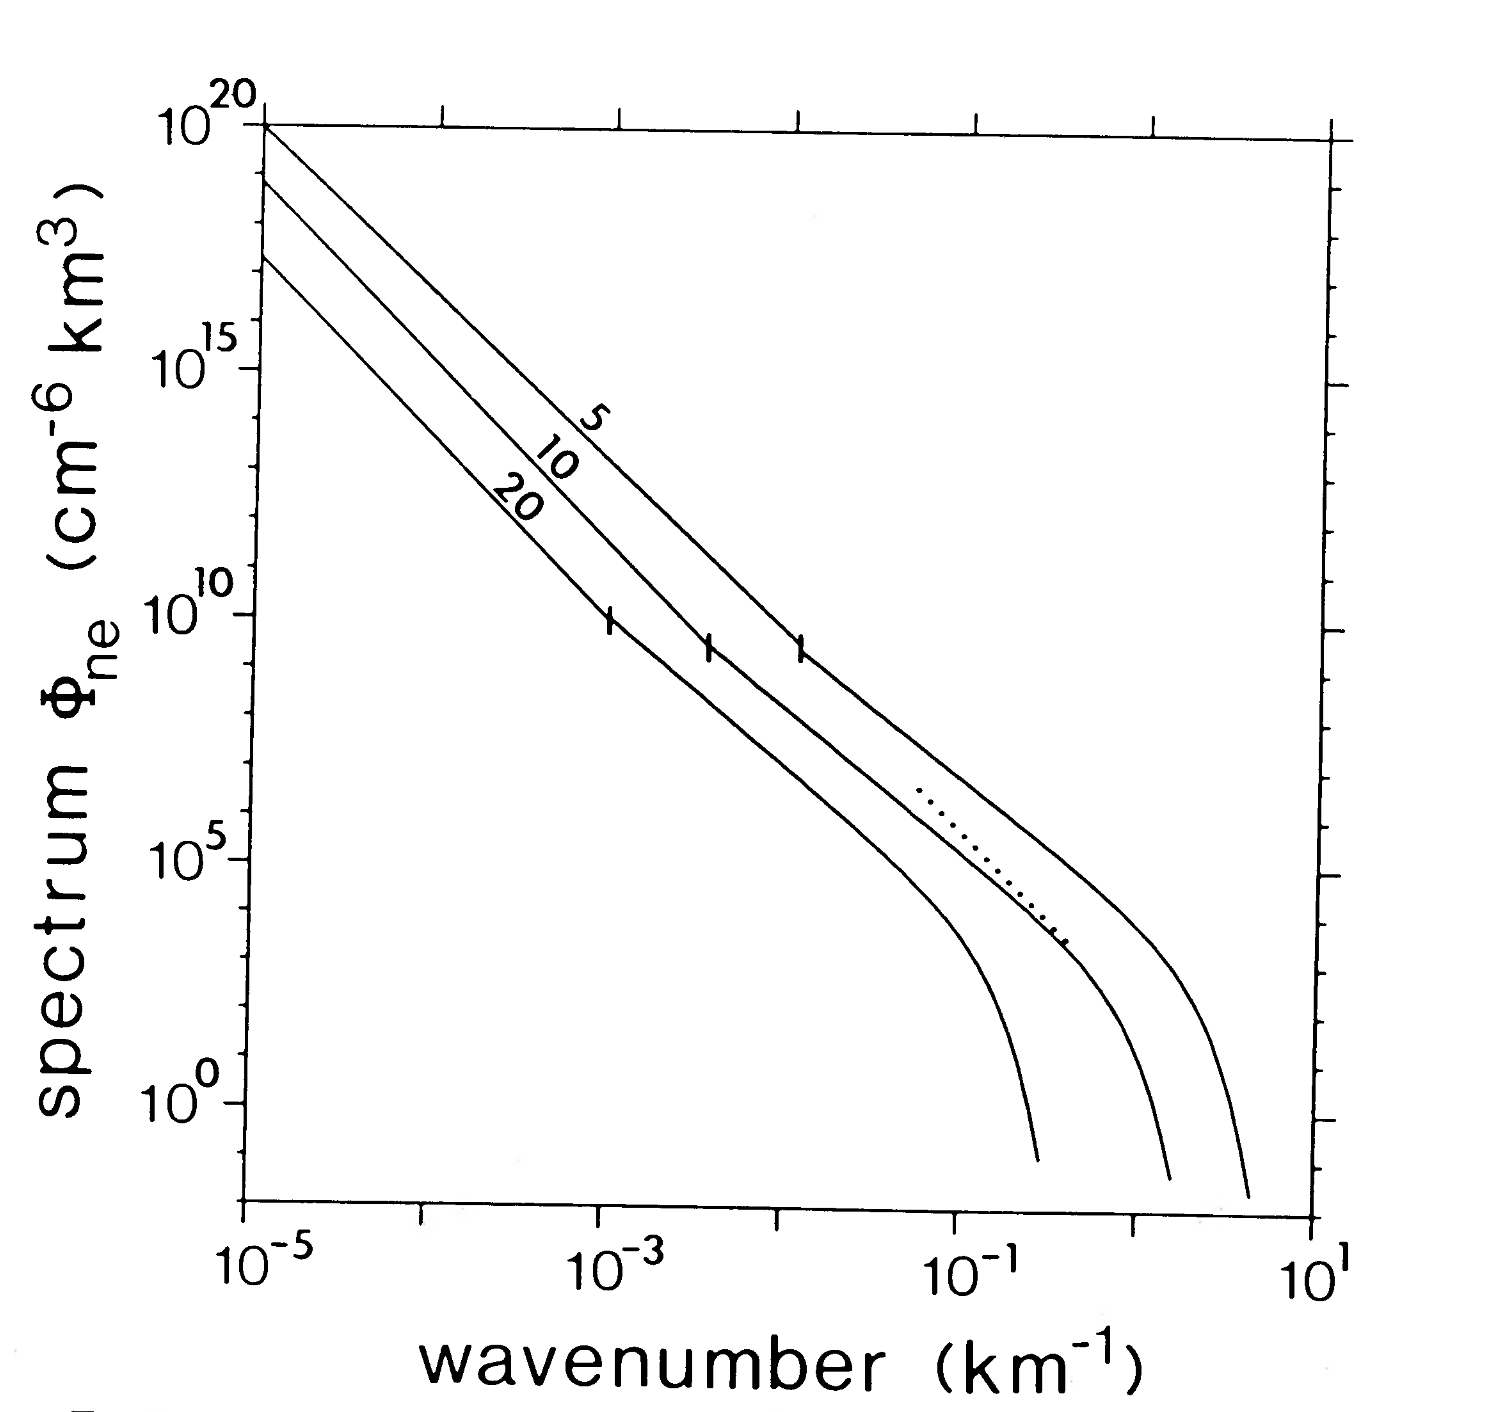
\includegraphics[width=\columnwidth]{coles_harmon_density_spectrum.png}
	\caption[Inferred spectrum of density fluctuations from \cite{Coles1989}]{Inferred spectrum of density fluctuations from \cite{Coles1989}. Black curves show the density fluctuation spectra at 5, 10 and 20 $R_\odot$. The vertical ticks indicate the wave number at which there is a break in the power law. The shape of these spectra is best described by a Kolmogorov like power law to some outer scale where a spectral flattening occurs, this shallower power law then continues until an inner scale where a rapid steepening is observed. The dotted line indicates a transient steeping seen in radar data from 1979.}
	\label{fig:CH_density_spectrum}
\end{figure}

Historically $S(\mathbf{q})$ was assumed to be isotropic however, recently it has been shown that this is not the case \citep{Kontar2019}. For an anisotropic spectrum of density fluctuations $S(\mathbf{q})$ can be written as 
\begin{equation}
S(\mathbf{q}) = S\left(\left[q_\perp^2 + \alpha^{-1}q_\parallel^2\right]^{1/2}\right),
\end{equation}
where $\alpha = h_\perp / h_\parallel$ is the ratio of perpendicular and parallel correlation lengths. \cite{Armstrong1990} find that the density inhomogeneities are elongated in the radial direction in a ratio of $\sim 3:1$ at 10 $R_\odot$, this would have the effect of a point source being observed as elongated in the perpendicular direction.

It is clear that a correct interpretation of radio observations provide a means to investigate the level of scattering and density fluctuation in the corona. Advances in radio astronomy over the past 40 years have lead to increased sensitivity, temporal resolution, frequency resolution and resolving power. Modern radio telescopes such as LOFAR, the Murchison Widefield Array \citep[MWA;][]{Lonsdale2009} and the upcoming Square Kilometre Array \citep[SKA;][]{Dewdney2009} are capable of observing the predicted spatial and time profiles of type IIIb bursts. That said, previous studies with LOFAR have tended to use tied-array imaging in this regard \citep{Kontar2017}, which has limited spatial resolution with respect to interferometric imaging.

Here I use LOFAR interferometric observations to determine the observed radio source size and position and how this differs from the expected source properties, which can be estimated from spectroscopy. %The discrepancy between what is observed and what is expected is used to determine the relative level of density fluctuations in the corona. 
Directly fitting interferometric visibilities provides an opportunity to observe low frequency radio sources at a spatial resolution in excess of what has usually been achieved. I compare these results with those of the tied-array observation from \cite{Kontar2017} and discuss the implication this may have on determining the relative level of density fluctuations in the corona. 
The remainder of this chapter is outlined as follows; an observation of a type IIIb burst is described in Section \ref{sec:obs}, in Section \ref{sec:data} I detail a method of directly fitting interferometric visibilities in order to recreate a sky brightness distribution and give results of observed source size. Section \ref{sec:data} also includes analysis of a type IIIb stria. I conclude with a discussion in Section \ref{sec:conclusion}.

\section{Observation} \label{sec:obs}
LOFAR is an interferometric array that spans across Europe observing radio frequencies at 10 - 240~MHz. 
An interferometric observation of the Sun, utilising 36 stations (24 core and 12 remote), was performed on 17 October 2015 from 08:00 UTC to 14:00 UTC. During this time, a type III solar radio burst was recorded  at 13:21 UTC. A calibrator source, Virgo A, was observed co-temporally in all subbands over the course of the observation.

Figure \ref{fig:context}a shows the X-ray flux measured by GOES for the duration of the LOFAR observation. A number of C-class flares can be seen in Figure \ref{fig:context}a but no significant activity is noticeable at the time of the radio burst, indicated by red vertical lines.

A dynamic spectrum of the burst was recorded in the LBA band by remote station RS509 and is shown in Figure \ref{fig:context}b. The inset shows a number of striations from 34 - 35~MHz and the white cross indicates the time and frequency at which the images described in Section \ref{sec:data} are made.

The maximum baseline of the LOFAR observation is 84\,km giving sub-arcminute resolution across almost all of the observed frequency range, offering an unprecedented level of spatial resolution.

\begin{figure}
    \centering
    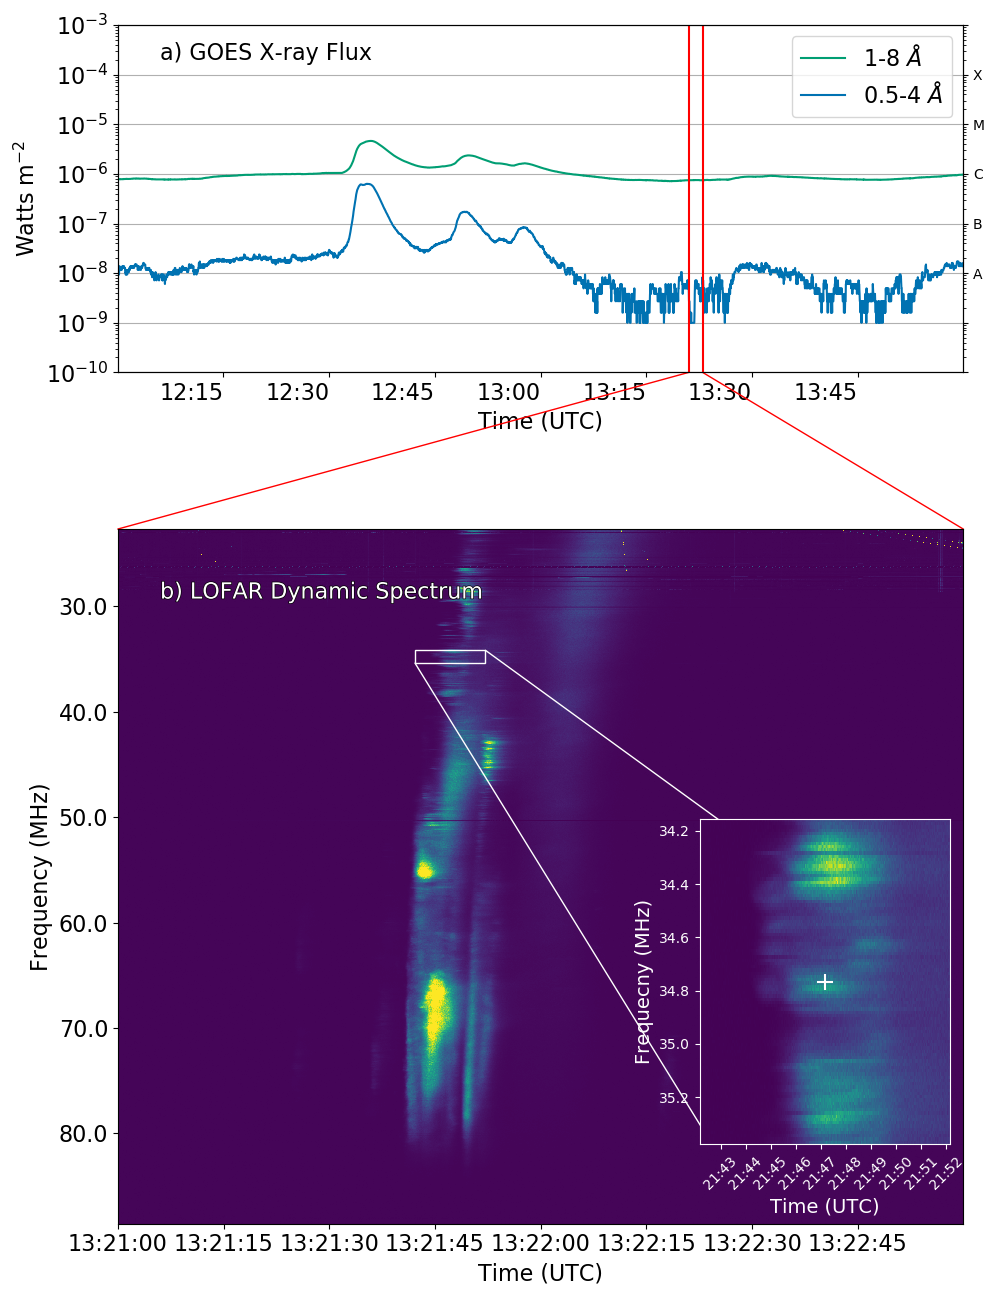
\includegraphics[width=\columnwidth]{Images/Burst_inset_goes_20200730.png}
    \caption[GOES X-ray lightcurves and dynamic spectrum for the duration of a LOFAR solar observation 17 October 2015.]{The X-ray light curve and radio dynamic spectrum for 17 October 2015. \textbf{a)} GOES X-ray lightcurves for the duration of the LOFAR solar observation. Minimal activity other than a number of C class flares prior to 13:00 UTC is observed. Red vertical lines indicate the time range of radio analysis. \textbf{b)} Dynamic spectrum of a type IIIb solar radio burst observed with LOFAR station RS509. The inset is a zoom of the region in the white box showing striation in the burst. The white cross indicates the time and frequency at which the images described in Section \ref{sec:data} are made.}
    \label{fig:context}
\end{figure}

\section{Data analysis and results} \label{sec:data}
The source sizes and positions of solar radio bursts in LOFAR data have typically been obtained by the ``tied-array imaging mode" \citep{Morosan2014} whereby a number of beams are tessellated across the Sun and the response in each beam is interpolated to produce an image \citep[e.g.][]{Reid2017,Kontar2017,Zucca2018, Morosan2019}. Tied-array imaging has the distinct advantage over interferometric observations in that it retains the ${\sim} 12$ kHz frequency resolution and ${\sim} 0.01$~s temporal resolution from LOFAR beamformed observations but it also contains a significant limitation. Tied-array observations can only be made using the LOFAR core stations as they share a single clock \citep{DeGasperin2019}, which makes it possible to add beamformed data coherently. This means that the maximum baseline from tied-array observations is approximately 2 km corresponding to an angular resolution of ${\sim} 17$~arcmin at ${\sim} 30$\,MHz. Not only this, but the effect of interpolation between each tied-array beam on the observed source size has not yet been compared to observations done interferometrically. It is therefore unclear whether previously observed source sizes are in fact due to the underlying source, or an effect of the imaging technique. Solar campaigns with LOFAR are now performed with a new mode which allow for simultaneous interferometric and tied-array observations. A detailed comparison of these modes is currently under study, which should resolve the ambiguity in source sizes determined with tied-array observations (Morosan, D. E. 2020, private communication). 
%a result of this interpolation or

In order to avoid such limitations of the tied-array mode, here we use interferometric observations from the LOFAR core and remote stations, offering a longer baseline of 84\,km and hence much better spatial resolution.
The LOFAR data from this observation were calibrated using the Default Preprocessing Pipeline \cite[DPPP;][]{VanDiepen2018} and a co-temporal observation of Virgo A. This corrects for effects such as antenna band-pass, clock drift and propagation effects through the ionosphere \citep{DeGasperin2019}. Correcting for antenna band-pass means accounting for the sensitivity of the LOFAR antennas at different frequencies (e.g. Figure \ref{fig:LBA_power_spec}). Clock drift occurs when the clocks on two different remote stations read slightly different times, this can introduce errors when the signals are correlated if the effect is not corrected. The ionosphere is an ionised medium and as such, radio waves propagating through it can be refracted and scattered, if these effects are not taken into account, the absolute position of an imaged source may be incorrect.
I next describe the technique of directly fitting the LOFAR visibilities to estimate radio source size and position.

To produce an image from interferometric observations, an inverse Fourier transform is performed on the observed visibilities, usually followed by a deconvolution of the array point spread function (PSF) from the resulting ``dirty-map" of the sky-brightness distribution.
For such a deconvolution, LOFAR uses an implementation of the multi-scale CLEAN algorithm known as WSClean \citep{Offringa2014}. In this procedure a weighting may be applied to the visibilities to improve sensitivity to various spatial scales, the most common of which is the Briggs robustness weighting scheme \citep{Briggs1995}. Recreating a radio image in this way can introduce artefacts depending on the Briggs robustness used, the number of iterations of the algorithm and a number of other parameters described in more detail in \cite{Hogbom1974, Cornwell2008, Offringa2014, Offringa2017} for example. These artefacts include changes to the source shape and size (see Figure \ref{fig:briggs_comparison} for an example). Therefore, to avoid ambiguity in the source size, shape and position due to such imaging algorithms, I directly fit the measured visibilities similar to a method used for X-ray observations using the Reuven Ramaty High Energy Solar Spectroscopic Imager \citep[RHESSI][]{Hurford2002, Kontar2010}. I describe this method in the following subsections. 

\subsection{Fitting the visibilities}
\label{sec:vis_fit}
The \textit{uv} plane is a Fourier space representation of antenna pair positions. Each point in the \textit{uv} plane is sensitive to emission of a particular angular scale. Due to the timescales over which type III bursts occur, solar observations are limited to a sparse sample of the \textit{uv} plane and techniques to increase samples in this plane, such as aperture synthesis, cannot be used. However, the large brightness temperatures of type III and type IIIb radio bursts \citep{Reid2014} give rise to a  high signal to noise ratio which allows a direct fit of a model to the visibilities.
In the following it is assumed that the emitting source is a single elliptical Gaussian. This is based on the dynamic spectrum in Figure \ref{fig:context}b, showing the type IIIb burst does not overlap any other bursts and as such is probably the only source in an interferometric image. The assumption leads to the convenient fact that an elliptical Gaussian in real space is observed as another elliptical Gaussian in the \textit{uv} plane. The form of this Gaussian is
\begin{equation}
V(u,v) = e^{-2\pi i(ux_0+vy_0)} \left( \frac{I_0}{2\pi} e^{-\left(\frac{\sigma_x^2(2\pi u^\prime)^2}{2}-\frac{\sigma_y^2(2\pi v^\prime)^2}{2}\right)} + C \right)
\label{eq:vis_gauss}
\end{equation}
where $x_0, y_0$ are the x and y coordinates of the source centre in real space, $\sigma_x, \sigma_y$ are the standard deviation in the x and y direction and $C$ is a constant background. Here the visibilities have been rotated to a new coordinate frame with axes $u^\prime$ and $v^\prime$ which are parallel and perpendicular to the major and minor axes of the Gaussian source such that $u^\prime = u\cos{\theta} - v\sin{\theta} \mbox{, } v^\prime = u\sin{\theta} + v\cos{\theta}$,  where $\theta$ is the angle of the major axis to the x axis, i.e. the position angle of the Gaussian on the \textit{uv} plane.

A nonlinear least squares fit is applied to the sample of visibilities in two stages. First, the source size, maximum intensity and angle relative to the x axis are found by fitting the absolute value of the complex visibilities also known as the amplitude.
In order to determine source location, the phase angle of the data is fit. Source location in real space determines fringe separation and orientation in Fourier space. The direct fitting of parameters to \textbf{$V(u,v)$} is then used to recreate the sky brightness distribution or image \textbf{$I(x,y)$}, which is the inverse Fourier Transform of Equation \ref{eq:vis_gauss}. The nonlinear least squares fit is implemented in the \texttt{lmfit} python library \citep{Newville2014} which uses the Levenberg–Marquardt algorithm to minimise the sum of least squares between the model, Equation \ref{eq:vis_gauss}, and the measured visibilities.

Although the computational time to perform a model fit to the visibilities is much less than creating a CLEAN image (10s of seconds compared to minutes) ensuring that the calibration was successful at a particular time and frequency is still a labour intensive process. Particularly bright radio emission from the Sun can corrupt the observation of the calibrator source making further calibration a futile effort. Thus, extending this analysis to a greater number of frequencies and times would 

Figure \ref{fig:uv_fit} shows the fit of the modelled Gaussian to the complex visibilities. Due to the fact that this fit is done in Fourier space, the amplitude and phase of the data and fit are shown in the \textit{uv} plane in Figure \ref{fig:uv_fit}a and \ref{fig:uv_fit}b respectively. Here, the points are the observed visibilities and the background colour map is the fit. In Figure \ref{fig:uv_fit}a a red ellipse indicates the full width at half maximum height (FWHM) of the fitted Gaussian. The fringes in Figure~\ref{fig:uv_fit}b show the fit of the source position to the distribution of visibility phases across \textit{uv} space.
Figure \ref{fig:uv_fit}c shows the increase in the amplitude of recorded visibilities with the angular scale on the sky that causes this increase. The red curves are where data points would lie for a Gaussian in visibility space with the FWHM in the major and minor direction obtained from the fit in Figure \ref{fig:uv_fit}a.

\begin{figure}
    \centering
    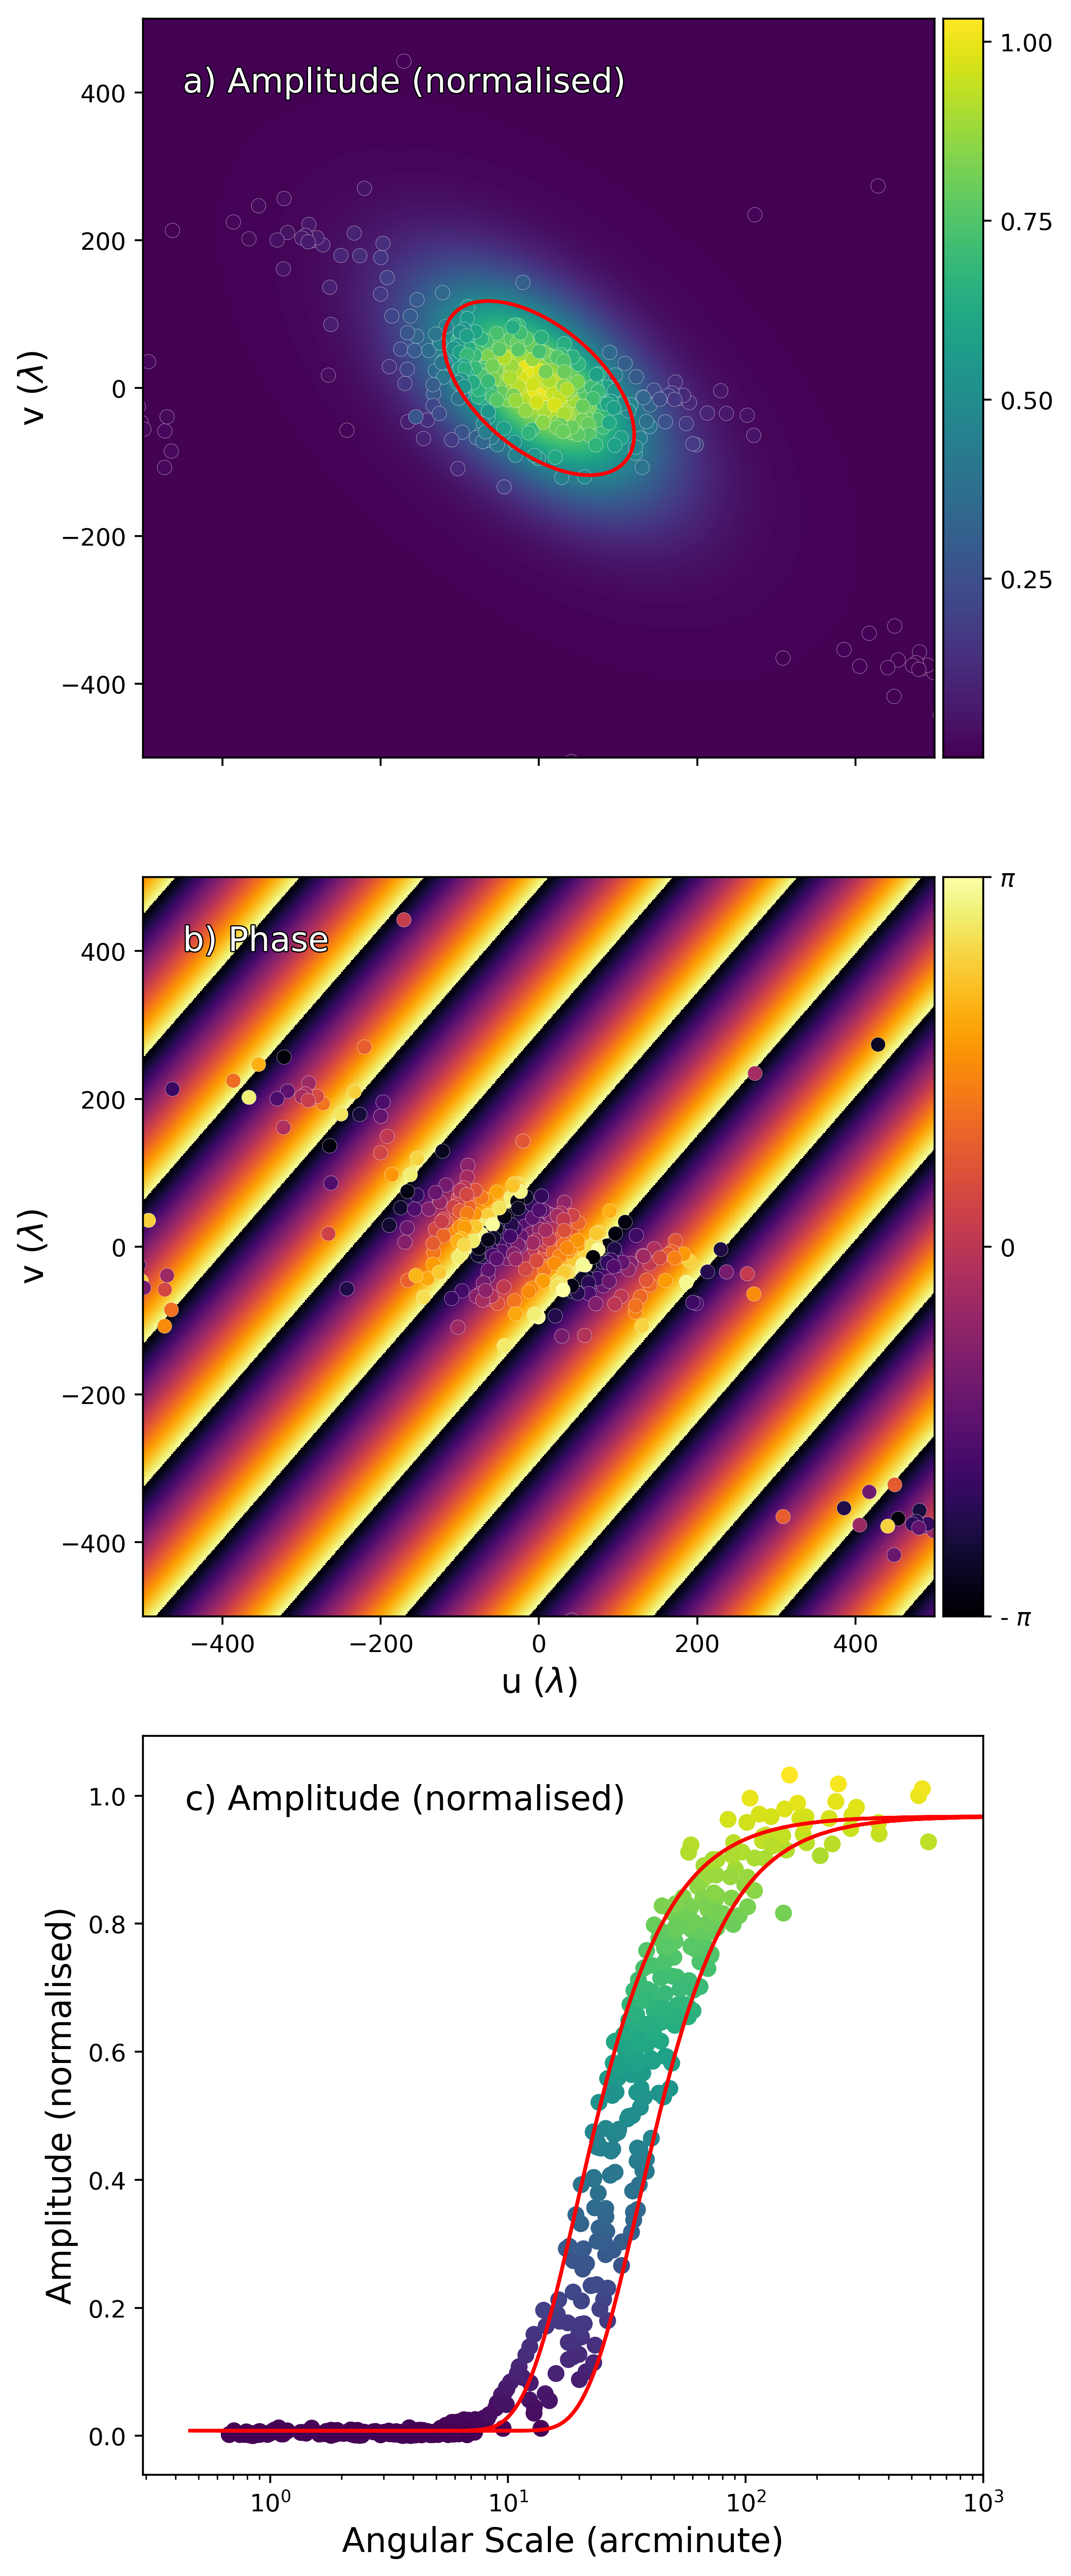
\includegraphics[width=0.5\columnwidth]{uv_fit_remote_20200826.png}
    \caption[Results of directly fitting LOFAR visibilities.]{Modelled visibilities determined from a direct fit to observed interferometric visibilities. \textbf{a)} Amplitudes of visibilities in the \textit{uv} plane for LOFAR observation. Background colour map shows a Gaussian fit. Red ellipse shows the FWHM of the normalised amplitude. \textbf{b)} Visibility phase in the \textit{uv} plane. Background colour map shows fitted phase angle. The fringe spacing is indicative of the distance of the source from the centre of the image while their orientation gives information on the source position. \textbf{c)} Visibility amplitudes received from different angular scales. Red curves indicate the FWHM of the semi-major and semi-minor axes of the fitted Gaussian.}
    \label{fig:uv_fit}
\end{figure}

The visibility fit reveals a source with a FWHM in real space of 18.8~arcmin $\pm 0.1$~arcmin and 10.2~arcmin $\pm 0.1$~arcmin, in the direction of the major and minor axis, respectively. The source is found at a position of $-1312^{\prime\prime}, -1064^{\prime\prime}$ from the solar centre giving a plane of sky distance of 1.75$\, R_\odot$. The parameters from the fit can then be used to recreate a sky-brightness distribution $I(x,y)$ in real space which is shown as contours over-plotted on a 171\,\AA~ image taken by the Atmospheric Imaging Assembly \citep[AIA;][]{Lemen2012} in Figure \ref{fig:recreate}. Note that, despite the theoretical high angular resolution of the long baselines afforded by LOFAR remote stations (84\,km), the source size is still large and there is little evidence of angular scales smaller than $\sim$10~arcmin in Figure~\ref{fig:uv_fit}c. I will discuss this further in Section \ref{sec:conclusion}.

\begin{figure}
    \centering
    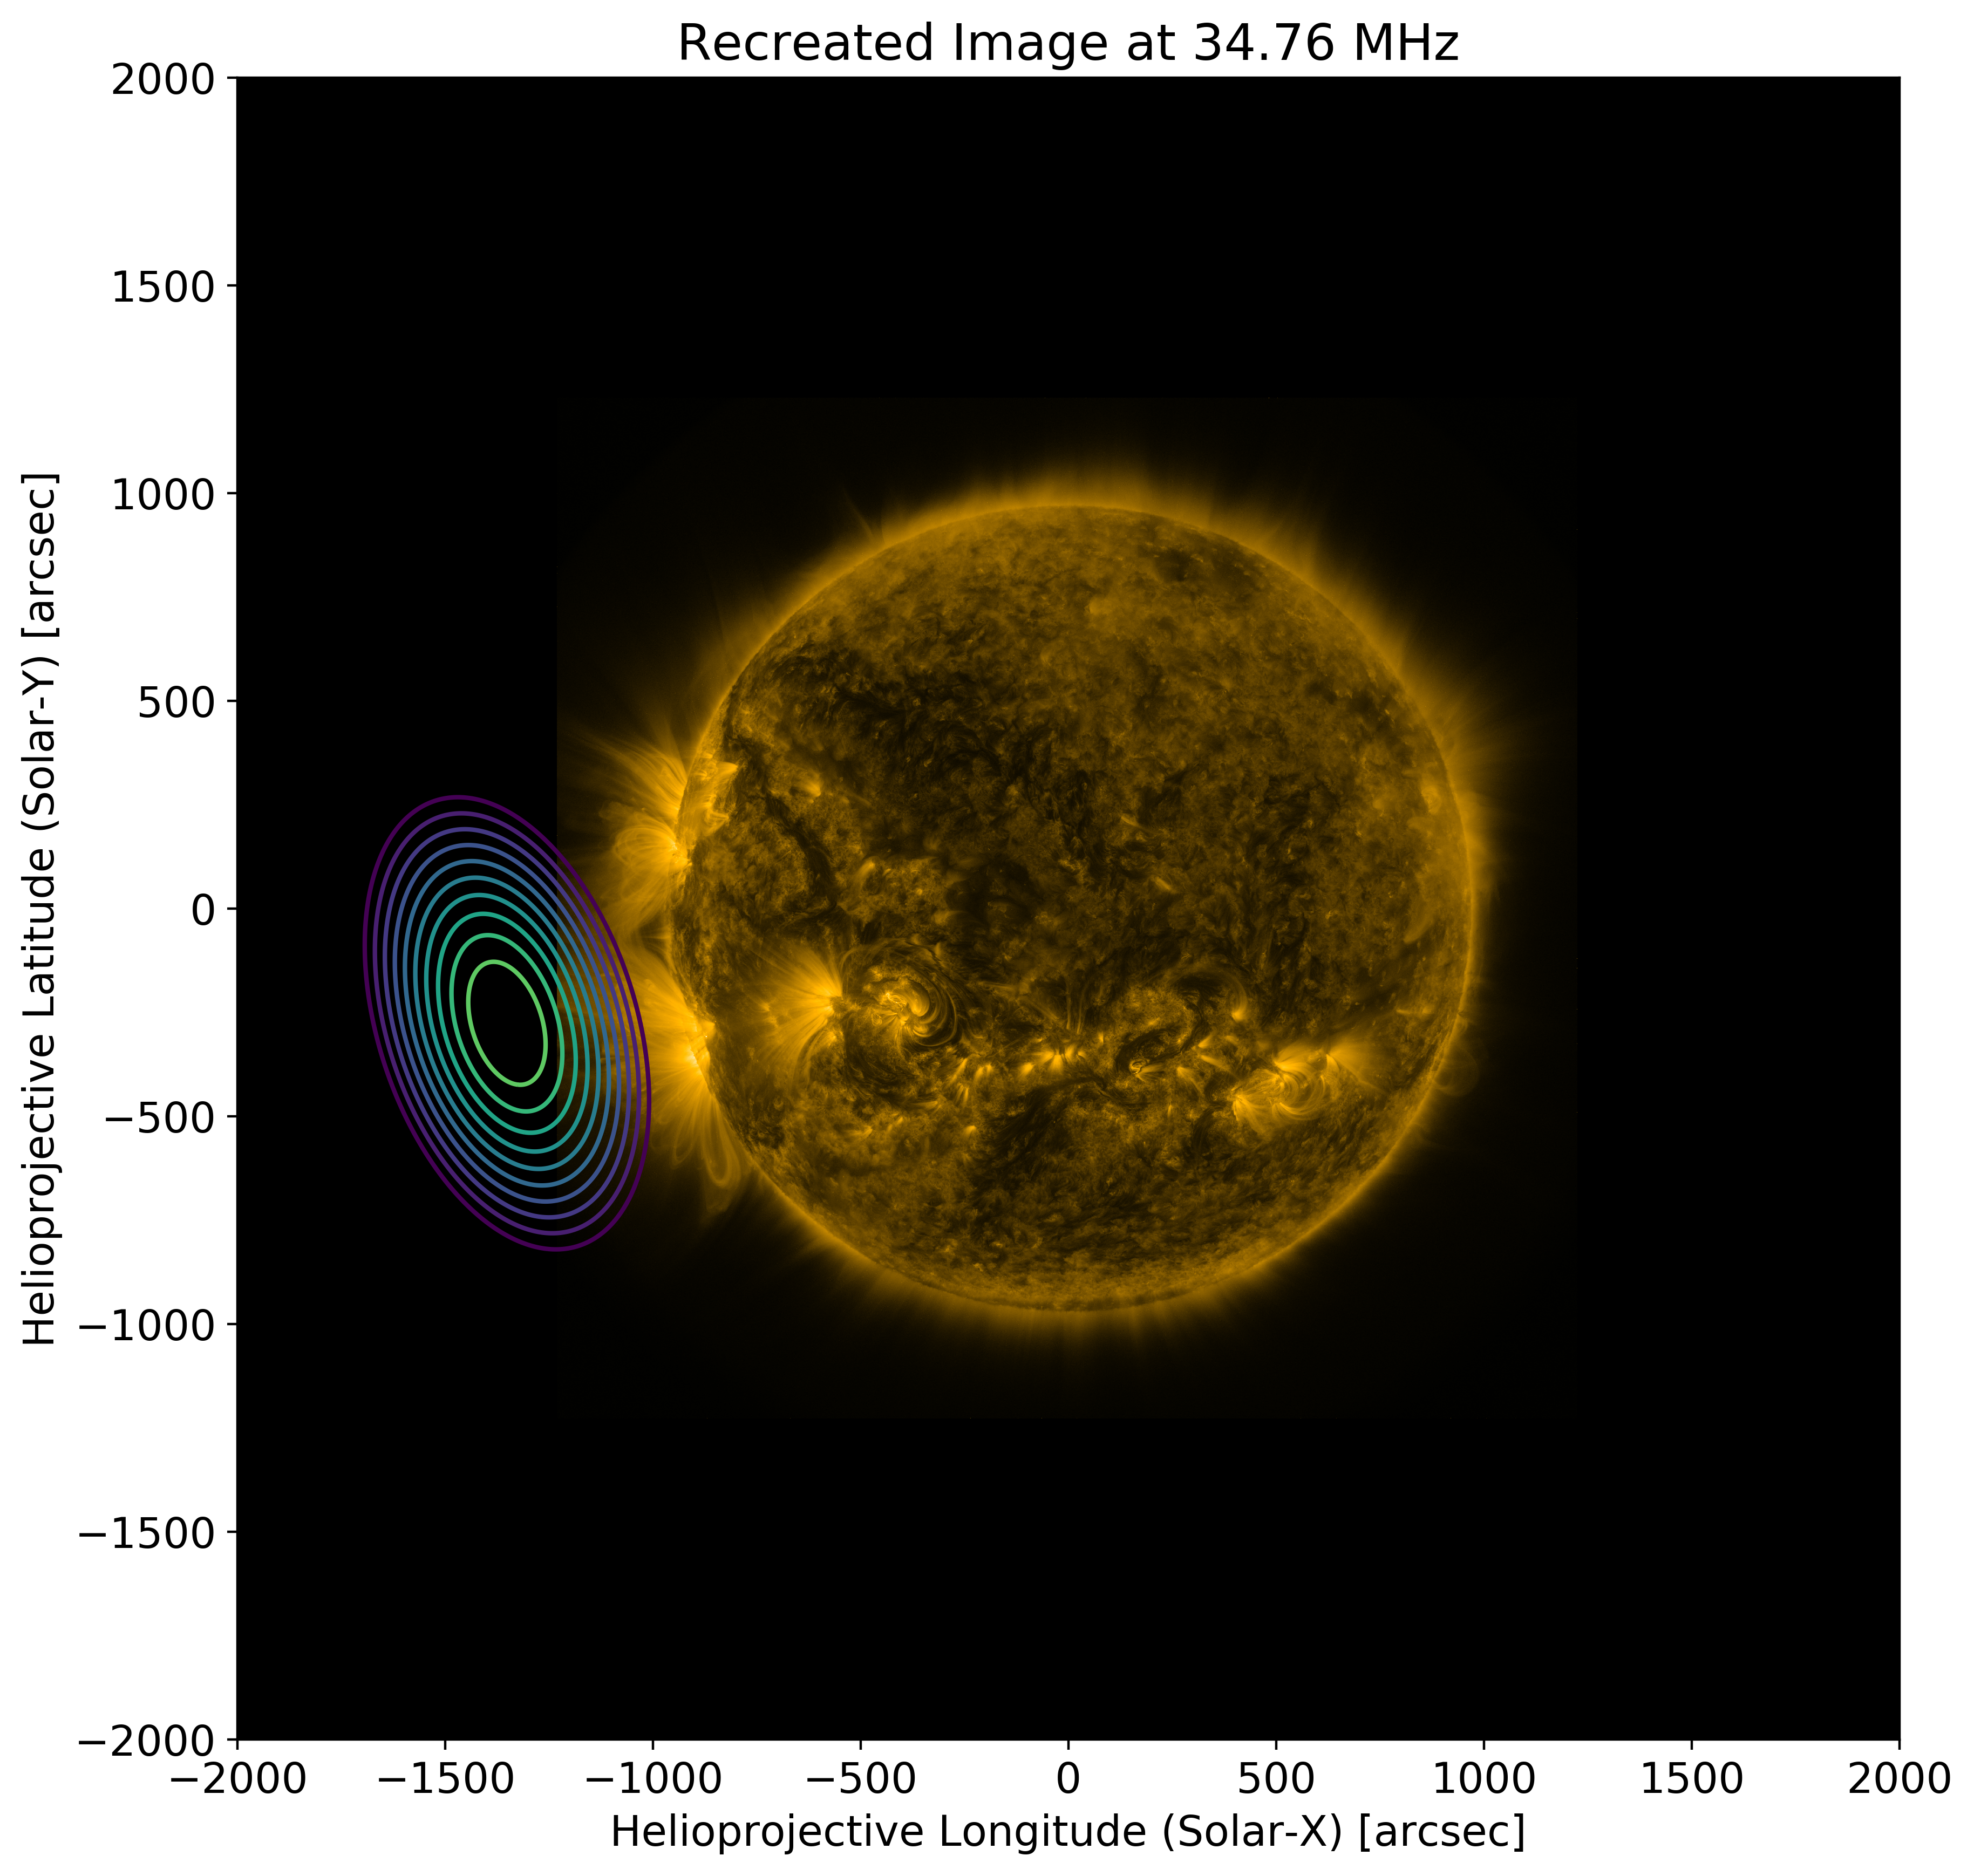
\includegraphics[width=\columnwidth]{im_recreate_remote_20200730.png}
    \caption[Recreated sky intensity profile of a type IIIb radio burst.]{Recreated sky intensity profile of a type IIIb radio burst occurring at 13:21:46 on 17 October 2015. The background solar image is an AIA 171$\AA$ image at 17 October 2015 13:21:46 UTC.} 
    \label{fig:recreate}
\end{figure}


\subsection{Type IIIb striae}
In the above I determined the source size and position using a direct modelling of LOFAR visibility observations. This provides us with an opportunity to compare the observed source size to its actual size, which can be estimated from spectroscopic observations, similar to the method of \cite{Kontar2017}.

To estimate the source size from spectroscopic measurements, I relate the FWHM of the frequency of the striation to its vertical extent in the solar corona $\Delta r {\sim} 2L \left(\Delta f/f\right)$ where $L$ is the characteristic density scale height \citep{Kontar2017} determined using a \cite{Newkirk1961} density model. Assuming emission occurs at the distance where the plasma frequency is $\sim 35$~MHz, this gives $L \approx 6200$~km.
A single striation was manually identified at 34.76~MHz from the dynamic spectrum. The time of maximum intensity for the burst was found and a vertical frequency slice was obtained from which $\Delta f/f$ was calculated. The individual striation, the centre of which is indicated by a white cross in the inset panel of Figure \ref{fig:context}b, was fit with a Gaussian. The value for $\Delta f$ of the striation was found from the FWHM of the fitted peak was found to be $\Delta f \sim 0.2$~MHz. The ratio of frequency to bandwidth for the striation was found to be $\Delta f/f = 0.006$, leading to an estimated source size of $3.18$~arcsec. 
Similar to \cite{Kontar2017}, this is far smaller than the source size observed from the visibility fit.

In the following section I will discuss why the most probable cause for the discrepancy in source size is radio scattering, as well as a discussion on the comparison of this observation to recent developments in the theory and the effect scattering has had on actual source size and position.

\section{Discussion}\label{sec:conclusion}

Adopting the theory described by \cite{Takakura1975} and used in \cite{Kontar2017}, the predicted source sizes of a type IIIb striation are much smaller than what is observed. The most probable cause for this discrepancy is a combination of radio light scattering in the solar corona, propagation effects in the Earth's ionosphere and limitations due to angular resolution.
With this observation we accounted for and corrected ionospheric effects in the calibration step \citep[Section \ref{sec:data} and ][]{DeGasperin2019} thereby removing the largest uncertainty in source size and position. By fitting the source size directly in visibility space we can directly see the power at which different angular scales were observed. The \textit{uv} coverage of this observation allows angular scales of ${\sim} 42$~arcsec to be observed (Figure \ref{fig:uv_fit}c) and although the predicted source size of ${\sim}3$~arcsec is smaller than this, the amplitude of the observed visibilities does not increase until ${\sim} 10$~arcmin indicating that this is, in fact, the smallest source size observed in the visibilities.

It should be noted that there is better \textit{uv} coverage along one axis compared to its orthogonal which may have an effect on the eccentricity of the elliptical Gaussian fit. However, owing to the qualitatively similar shape as predicted by \cite{Kontar2019} for a burst originating near the solar limb, I am confident that the eccentricity is representative of the real source. The orientation and elongation of the source are also consistent with observations of anisotropic scattering in the solar wind \citep{Anantharamaiah1994, Ingale2015} where scattered sources are elongated perpendicular to the large scale (radial) magnetic field of the Sun.

Having accounted for all systematic effects that can affect the source size, I conclude that the large source sizes observed in this observation are due to the effect of scattering in the solar corona only. Previous tied-array observations have similar conclusions, however the tied-array technique interpolates data from a tessellation of beams across the Sun, and this introduces an ambiguity to the origin and size of sources. 
I assume the origin of the radio source to be somewhere above the active regions close to the East limb. 
An exploratory potential free source surface (PFSS) extrapolation suggests open field lines at an angle of $ \theta_s {\sim} 20^\circ$ from the plane of sky towards the observer. Similar to \cite{Chrysaphi2018} (Equations 5 and 6), an out-of-plane heliocentric distance for the source can be determined. Using the observed in-plane heliocentric distance and an angle of $ \theta_s {\sim} 20^\circ$ from the plane of sky, I obtain an out-of-plane heliocentric distance of 1.82$\, R_\odot$. Comparing this to Figure 8 in \cite{Kontar2019}, which shows the effect of the angle from the plane-of-sky $\theta_s$ on source position and FWHM size in the major and minor axis, one would expect a ratio of the FWHM on the minor axis to the FWHM of the major axis to be of the order of 0.6. These observations show a ratio of 0.54 suggesting $ \theta_s {\sim} 20^\circ$ is an appropriate approximation for the angle from the plane-of-sky.

The FWHM of the source at 34.76~MHz along the major and minor axis for this observation are $18.8$~arcmin $\pm 0.1$~arcmin and $10.2$~arcmin $\pm 0.1$~arcmin respectively. This gives the FWHM area of the source to be $A_s = 150.6~\mbox{arcmin}^2$, which I note is smaller than that of \cite{Kontar2017} who measure $A_s = 400~\mbox{arcmin}^2$ at a similar frequency of 32.5~MHz. While this could be simply due to these being two separate observations, this may be more indicative of a discrepancy between source sizes measured in interferometric observations and tied-array observations.
As mentioned in Section~\ref{sec:data}, the spatial resolution of LOFAR interferometric observations is superior to that of tied-array observations. This is mostly due to the additional stations that can be used for interferometric imaging and thus greater baseline lengths, but also due to the way tied-array images are made. Tied-array observations is carried out by pointing a number of beams in a honeycomb like pattern centred on the Sun and interpolating data from each of the tessellated beams. The effect of this on observed source sizes and position is, as of yet, un-characterised. \cite{Kontar2017} attribute the large source size observed in their tied-array observation of a type IIIb radio burst to the scattering of radio waves off of density inhomogeneities in the solar corona. It was later determined that a relative rms fluctuation of electron density of $\varepsilon = 0.8$ was necessary to explain the large source size observed \cite{Kontar2019}. While it is evident that radio wave scattering causes radio bursts to appear larger in observations than predicted, the reduced spatial resolution of tied-array imaging may result in an overestimate of $\varepsilon$.

The last decade has seen a renewed interest in low frequency observations of the radio sun with state of the art radio interferometers such as LOFAR and the MWA. Radio bursts emitted via the plasma emission process give a diagnostic of the local plasma density which may give insight into the turbulent nature of coronal plasma. It is theorised that the size of low frequency radio emission is limited by scattering caused by turbulence \citep{Bastian1994}, however it is only recently that the angular resolution necessary to challenge this theory has become available. In particular, a robust comparison of sources observed with tied-array and interferometric imaging is needed. Analytical approximations of radio scattering \citep[e.g.][]{Chrysaphi2018,Gordovskyy2019,Sharma2020} have seen some success in accounting for apparent source shift and brightness temperature due to scattering, however they cannot account for the anisotropic nature of scattering and may not be appropriate to describe large angle scattering near the source location. As such, a full numerical treatment of scattering \citep[e.g.][]{Thejappa2008, Bian2019, Kontar2019}, in combination with interferometric imaging, is necessary to fully understand radio wave propagation in the turbulent coronal plasma. In order to definitively determine $\varepsilon$, more information on the power spectrum of density fluctuations and the scales on which radio scattering most effectively occurs is needed.

\section{Conclusion}
In summary, a type IIIb radio burst was observed with LOFAR on 17 October 2015 at approximately 13:21:00 UTC. The bandwidth of an individual striation at 34.76~MHz suggests a FWHM source size of $3.18$~arcsec. Directly fitting visibilities to avoid effects of deconvolution algorithms reveals a FWHM source size in the major and minor axes of $18.8$~arcmin $\pm 0.1$~arcmin and $10.2$~arcmin $\pm 0.1$~arcmin respectively. The source is located at $-1312^{\prime\prime}, -1064^{\prime\prime}$ from the solar centre. 
Having corrected for radio wave propagation in the ionosphere, I conclude that scattering from electron density fluctuations in the solar corona is the main cause of source broadening. I discuss how values for the rms relative electron density fluctuations determined from numerical models and compared to tied-array observations may be an overestimate. 
In the future, a combination of remote observations from LOFAR and \textit{in situ} measurements of plasma properties from PSP and Solar Orbiter \citep{Muller2013,Muller2020} at a variety of heliocentric distances in the corona and solar wind will be needed to form a more complete picture of coronal turbulence.